\begin{appendices}
\chapter{Variant maps with hypercomplementation}
\label{apdx:maps}
As was shown in chapter 3 section~\ref{sec:hypercomp}, phylogenetic analysis of \gene{UBE2I} and \gene{SUMO1} both showed that variants with ability to complement yeast better than wild-type are likely deleterious in humans. Thus, fitness scores were transformed so that such hypercomplementing mutations are considered to be deleterious. However, since hypercomplementing substitutions may provide interesting clues about differences between yeast and human cellular contexts, the untransformed versions the maps are provided below.

\begin{landscape}
\begin{figure}[h]
	\centering
	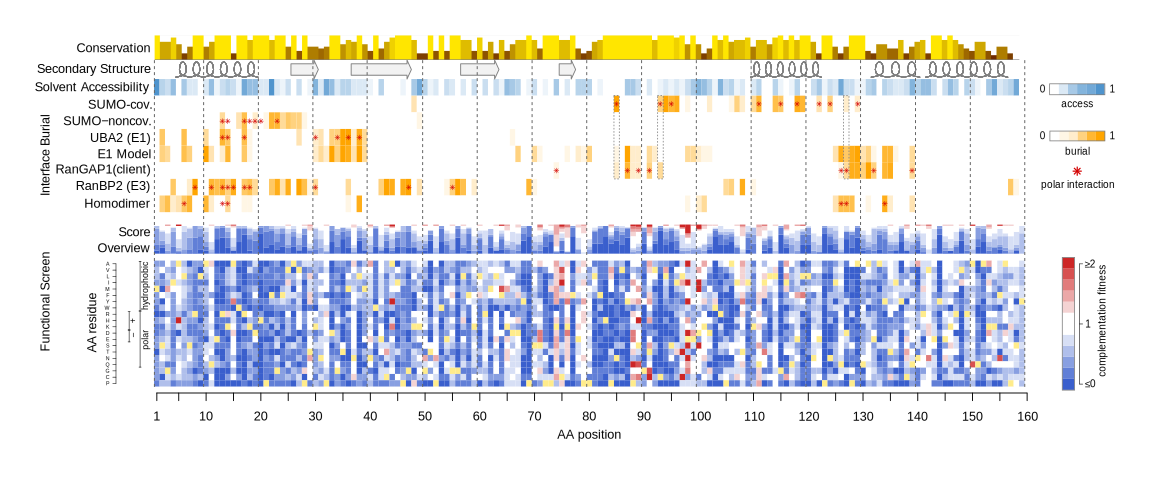
\includegraphics[width=9in]{img/ube2i_map.pdf}
	\caption{Functional map of UBE2I. From top to bottom: Position-wise evolutionary conservation (AMAS); Secondary structure; Relative solvent accessibility; Relative burial in protein-protein interaction interfaces with covalently bound SUMO, non-covalently bound SUMO, the SUMO E1 complex at two different stages of activation, the sumoylation substrate RanGAP1, the E3 RanBP2, and the UBE2I homodimer; A summary track showing the relative number of amino acid changes resulting in different fitness effects; and finally the individual amino acid change effects sorted by physicochemical groups.}
\end{figure}
\end{landscape}


\begin{landscape}
\begin{figure}[h]
	\centering
	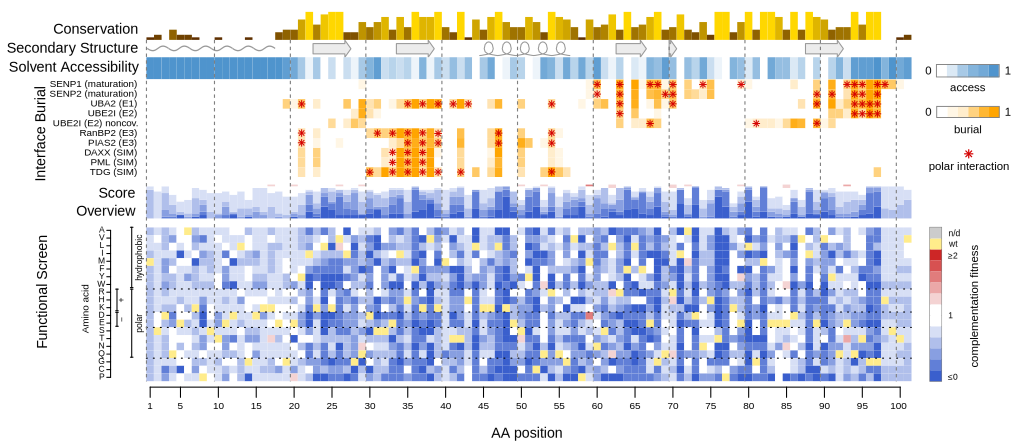
\includegraphics[width=9in]{img/sumo1_map_noflip.pdf}
	\caption{Functional map of SUMO1. From top to bottom: Position-wise evolutionary conservation (AMAS); Secondary structure; Relative solvent accessibility; Relative burial in protein-protein interaction interfaces with SENP proteases, E1 complex, covalent and noncovalent E2 binding, E3s and three different SIM motifs; A summary track showing the relative number of amino acid changes resulting in different fitness effects; and finally the individual amino acid change effects sorted by physicochemical groups.}
\end{figure}
\end{landscape}


\begin{landscape}
\begin{figure}[h]
	\centering
	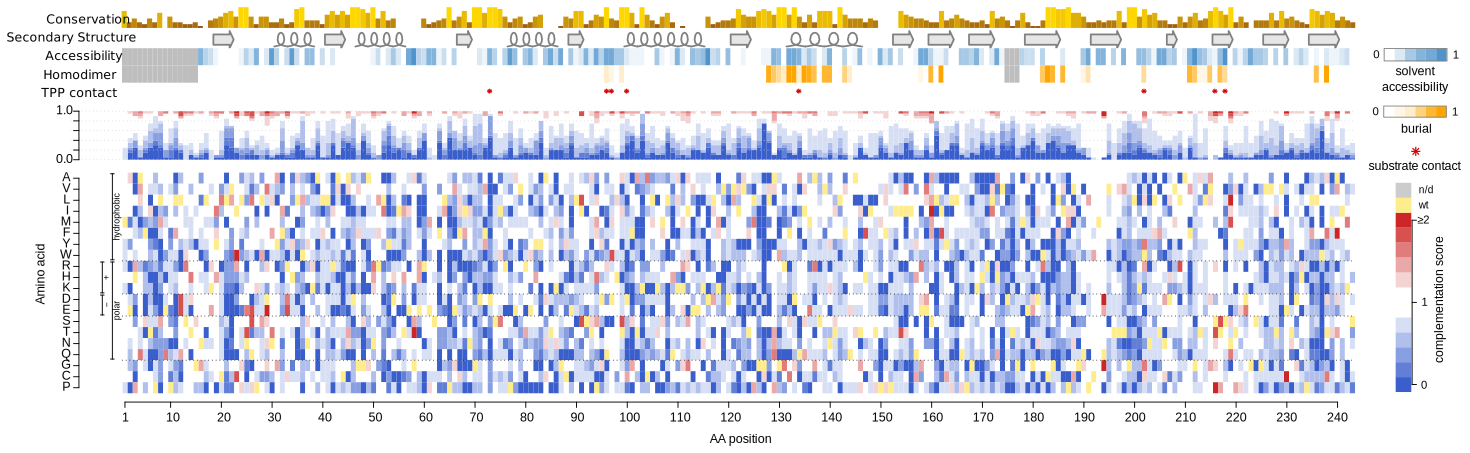
\includegraphics[width=9in]{img/tpk1_map_noflip.pdf}
	\caption{Functional map of TPK1. From top to bottom: Position-wise evolutionary conservation (AMAS); Secondary structure; Relative solvent accessibility; Relative burial in homodimerization interfaces; Positions contacting the Thiamine pyrophosphate (TPP) molecule; A summary track showing the relative number of amino acid changes resulting in different fitness effects; and finally the individual amino acid change effects sorted by physicochemical groups.}
\end{figure}
\end{landscape}


\begin{landscape}
\begin{figure}[h]
	\centering
	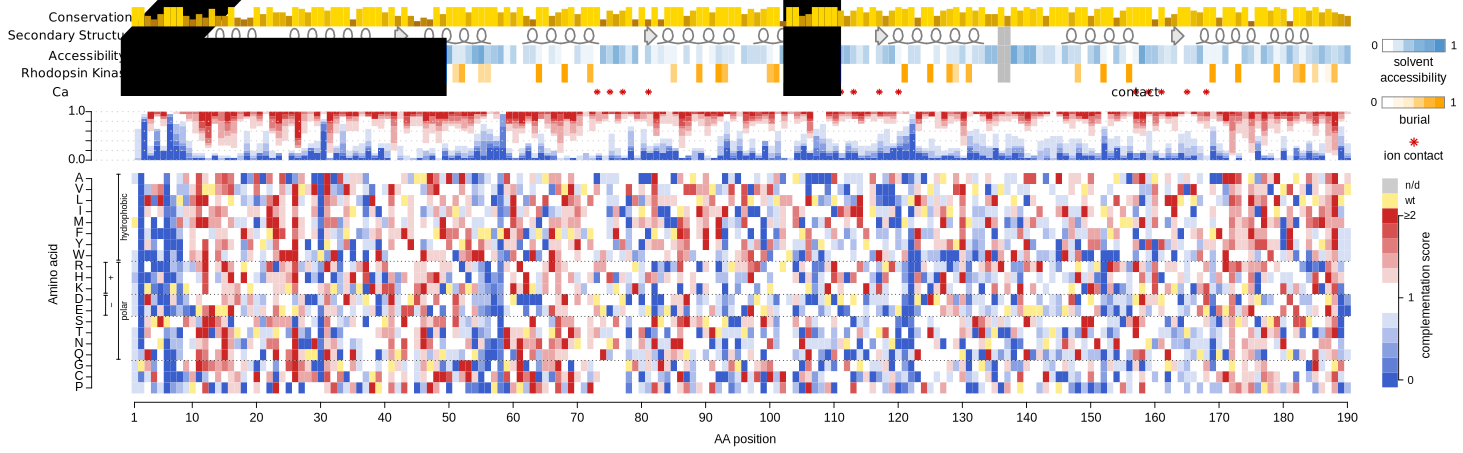
\includegraphics[width=9in]{img/ncs1_map_noflip.pdf}
	\caption{Functional map of NCS1. From top to bottom: Position-wise evolutionary conservation (AMAS); Secondary structure; Relative solvent accessibility; Relative burial in interaction interface with rhodopsin kinase; Positions contacting Calcium ions; A summary track showing the relative number of amino acid changes resulting in different fitness effects; and finally the individual amino acid change effects sorted by physicochemical groups.}
\end{figure}
\end{landscape}


\begin{landscape}
\begin{figure}[h]
	\centering
	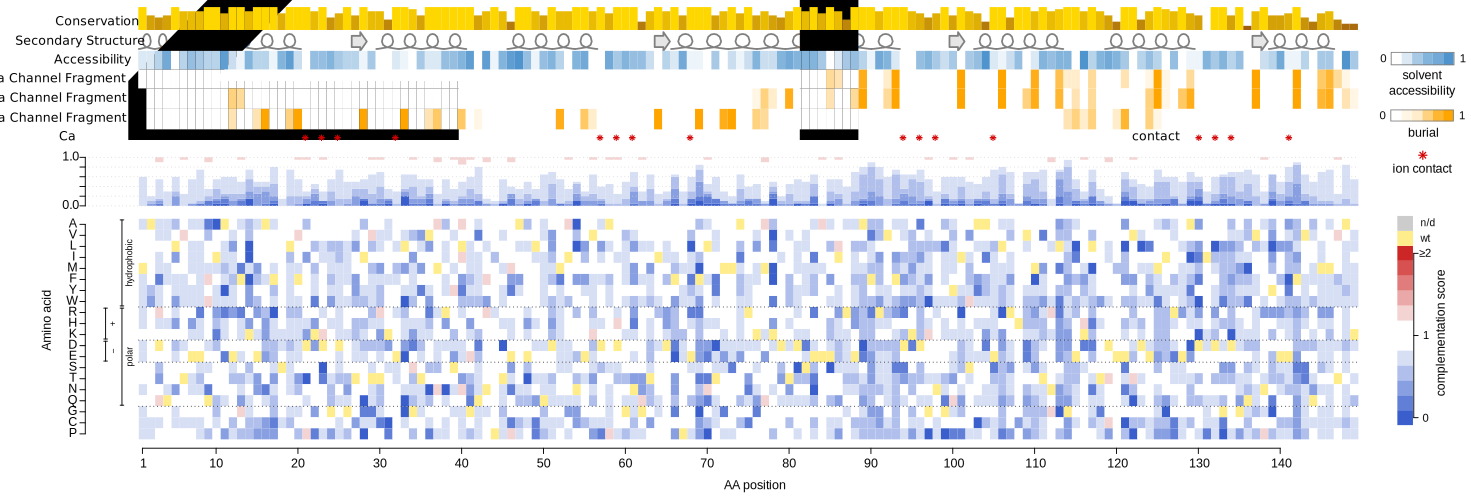
\includegraphics[width=9in]{img/calm1_map_noflip.pdf}
	\caption{Functional map of Calmodulin. From top to bottom: Position-wise evolutionary conservation (AMAS); Secondary structure; Relative solvent accessibility; Relative burial in interaction interface with ion channel fragments; Positions contacting Calcium ions; A summary track showing the relative number of amino acid changes resulting in different fitness effects; and finally the individual amino acid change effects sorted by physicochemical groups.}
\end{figure}
\end{landscape}

\end{appendices}